\chapter{Algoritmy strojového učení pro detekci anomálií}
\label{ml-algoritmy}

Strojové učení se dělí na~dvě základní kategorie. Těmito jsou učení s~učitelem, a učení bez~učitele \cite{data-science-concepts-and-practice}. Učení s~učitelem funguje na~tom principu, že se algoritmu předají již anotovaná data~\cite{data-science-concepts-and-practice}. Dopředu je známo, kolik a jaké třídy existují a jak vypadají typická data takové třídy. Na~základě těchto dat, jimž se říká trénovací, dokáže algoritmus vytvořit model schopný rozřazovat nově příchozí neznámá data do~daných tříd~\cite{data-science-concepts-and-practice}. Pro~detekci anomálií to lze použít v~případech, kdy se dobře ví, jaké anomálie mohou nastat a jak tyto vypadají. Poté se již jen neznámá data předají modelu, jenž se rozhodne, zda se jedná o~anomálii či nikoliv.

U~učení bez~učitele se ztrácí komfort označených dat. Algoritmy dopředu neví, jaké třídy existují, a typicky je jejich úkolem data na~základě jistého druhu podobnosti do~nějakých tříd rozdělit~\cite{data-science-concepts-and-practice}. Za~tímto účelem algoritmy vyžadují určité parametry, dle kterých rozdělovat. Častým je například právě počet tříd, do~nichž data rozdělit. Vzhledem k~dopředné neznalosti dat tu většinou nedochází k~trénování nějakého modelu, nýbrž výpočet probíhá nad všemi vstupními daty~\cite{supervised-vs-unsupervised-learning}. Anomálie se poté detekují tím způsobem, že z~nalezených tříd některá právě anomální data vyčnívají, nebo se do~žádné třídy ani nepřiřadí.

K~detekci anomálií se typicky používá učení bez učitele~\cite{intro-to-anomaly-detection}, jímž se také práce zabývá, a to z následujících důvodů. Vzhledem k~tomu, že anomálie se dějí velmi zřídka, neboť pokud by byly pravidelné, již by se jednalo o~standardní chování, tak je velmi těžké nasbírat trénovací data~\cite{intro-to-anomaly-detection}. V~mnoha případech užití, mezi kterými je i například právě monitorování systémů, by se modely musely s~příchodem nových dat v~čase neustále přetrénovávat, což je nepraktické. Učení bez učitele tyto problémy řešit nemusí. Pokud se navíc objeví zcela nový typ anomálie, algoritmy učení s~učitelem anomálii nedokáží rozpoznat, neboť taková data při~trénování neviděly~\cite{intro-to-anomaly-detection}. Algoritmus učení bez učitele tuto detekovat dokáže, protože vidí pouze vybočující data od~standardu a nesnaží se je nijak kategorizovat do~třídy \uv{anomálie}.

Pro~shrnutí, jestliže se předem ví, co přesně detekovat a jak to vypadá, je vhodné použít učení s~učitelem. Natrénuje se model, který bude poměrně rychle určovat, zda je jeho vstup anomální, či nikoliv. Pokud však dopředu nejsou anomálie zcela známé, mohou se měnit v~čase, nelze je kategorizovat, je zapotřebí učení bez učitele.

V~případě RQA je jedinou cestou učení bez~učitele, neboť o~datech neexistuje žádná dopředná znalost. Trénovací dataset by pro~učení s~učitelem šlo vytvořit pouze manuálním průchodem a vyčleněním anomálií z milionů logů nebo vhodným použitím právě učení bez~učitele. Neustálý příchod nových dat by znamenal nutnost pravidelného přetrénování. Natrénovaný model by navíc musel tisíce nově příchozích logů zpracovávat samostatně, zatímco algoritmus učení bez učitele to provede v~jediném výpočtu. Nadcházející sekce se zabývají různými typy algoritmů učení bez učitele, jejich zástupci a způsobem využití pro~detekci anomálií.

\section{Shluková analýza}
Shluková analýza slouží k~rozdělení neznámých dat do~shluků. Prvky těchto shluků, nebo také tříd, si pak jsou v~určitých aspektech podobné. Anomálie lze rozpoznat podle topologie shluků nebo tím, že některý prvek žádnému shluku ani nebyl přiřazen.

\subsection{Kategorizace algoritmů}
Existuje několik způsobů členění shlukových algoritmů. To znamená, že jeden algoritmus může spadat do~více skupin. V~následujících sekcích jsou uvedeny nejběžnější kategorie.

\subsubsection{Rozdělovací algoritmy}
V~anglické terminologii jsou jinak označovány jako \uv{centroid-based} algoritmy~\cite{cluster-methods-article}. Jedná se o~algoritmy, které data rozdělí do~předem stanoveného počtu tříd. Na~začátku se pro~každou třídu určí její centrální bod, ke~kterému se poté ostatní body přidružují na~základě třeba vzdálenosti či jiných parametrů~\cite{cluster-methods-article}. Do~této kategorie spadají například K-Means, SOM nebo jistým způsobem i GMM. Tyto algoritmy přiřadí všechny prvky nějakému shluku. Z~toho důvodu nejsou schopny odhalit jednotlivé outliery, nicméně dokáží rozpoznat celý anomální shluk.

\subsubsection{Hierarchické algoritmy}
Na rozdíl od~rozdělovacích algoritmů, které rovnou počítají se všemi daty, pracují hierarchické algoritmy tak, že shlukování provádí nad~podmnožinami datasetu~\cite{cluster-methods-article}. Tím se získají částečné shluky, které lze dále spojovat do~větších například aglomerativními metodami (single/complete linkage) \cite{cluster-methods-article}. Vznikne tak hierarchický strom shluků, nebo-li dendrogram~\cite{cluster-methods-book, cluster-methods-article}.
Typickým představitelem je kupříkladu HDBSCAN.

\subsubsection{Algoritmy založené na~hustotě}
U~těchto algoritmů se shluky vytvářejí na~základě hustoty bodů v~prostoru. Jejich velkou výhodou je to, že dopředu není nutno znát počet tříd, do~kterých se data rozdělují~\cite{cluster-methods-book}. Dokonce nemusí dostatečně odlehlá data přiřadit žádné třídě~\cite{cluster-methods-book}. To znamená, že jsou schopny relativně snadno detekovat šum. K~těmto metodám se řadí DBSCAN, HDBSCAN nebo OPTICS.

\subsubsection{Algoritmy založené na~pravděpodobnostním rozložení}
Tyto algoritmy jsou také občas označované jako \uv{algoritmy založené na~modelech}, kde se modelem typicky myslí pravděpodobnostní rozložení~\cite{cluster-methods-book}. Shluky jsou zde definované jako objekty patřící do~stejného rozložení~\cite{cluster-methods-book}. Nejčastěji používaným rozložením je Gaussovo a algoritmem proto GMM.

\subsection{K-Means}
Jedná se o rozdělovací algoritmus shlukující všechna data do~předem stanoveného počtu tříd. Kniha \emph{Data Science: Concepts and Practise}~\cite{data-science-concepts-and-practice} popisuje algoritmus následovně:

\begin{enumerate}
    \item Z~dat se náhodně vybere tolik bodů, kolik je tříd, a ty slouží jako centrální body.
    \item Vypočítají se vzdálenosti všech bodů od~každého centrálního bodu a přiřadí se k~tomu s~nejmenší vzdáleností.
    \item Spočítá se střed každého shluku, který se stává jeho novým centrálním bodem.
    \item Pokud žádný bod nezměnil třídu, algoritmus končí, jinak se opakuje od~bodu 2.
\end{enumerate}

Dále lze v knize najít několik běžně používaných typů vzdáleností. Nejrozšířenější je Eukleidovská vzdálenost, nebo-li délka úsečky mezi dvěma body. Další je Manhattanská vzdálenost, která měří cestu k~cíli pouze po~pravoúhlých cestách a jež si své jméno vydobyla podle cestování po~New Yorku. Chebyshevova vzdálenost zase udává maximální rozdíl mezi všemi atributy datasetu. V~případě obrázku~\ref{k-means-img}(b) je to maximum z [(3 - 1), (1 - 2)] = 2. 

\begin{figure}[tbh]
    \centering
    \subfloat[\centering Shlukování dat algoritmem K-Means]{{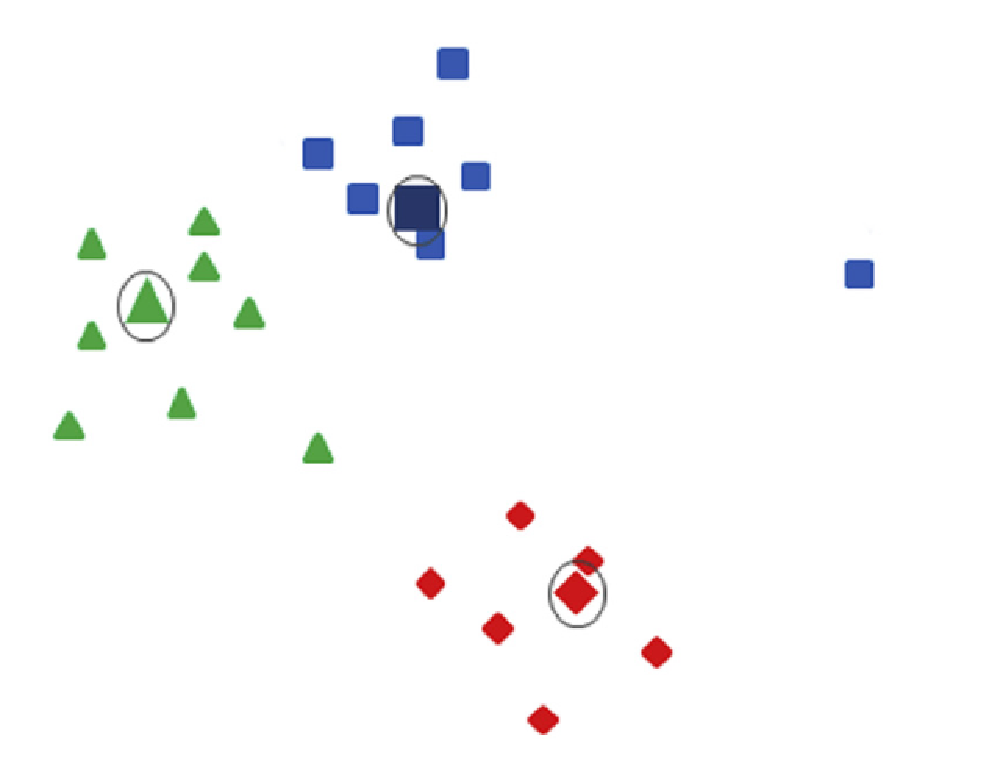
\includegraphics[width=7cm]{obrazky/k-means.pdf} }}
    \qquad
    \subfloat[\centering Typy vzdáleností používané v~K-Means]{{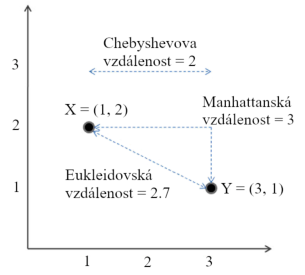
\includegraphics[width=7cm]{obrazky/distances.pdf} }}
    \caption{Výsledek algoritmu K-Means a různé typy vzdáleností (upraveno z \cite{data-science-concepts-and-practice})}
    \label{k-means-img}
\end{figure}

\subsection{GMM}
GMM (Gaussian Mixture Model), nebo-li směs Gaussových rozložení, je jeden z~nejvýznamnějších algoritmů strojového učení. Mimo shlukování ho lze využít i pro~klasifikaci. Jako se u~K-Means na počátku zvolí centrální body, tak tu se vytvoří určitý počet normálních rozložení. Body se poté jednotlivým rozložením přiřazují (viz. obr.~\ref{gmm-img}) a po~dokončení jednoho cyklu se přepočítají jejich parametry, tedy střed a kovarianční matice~\cite{sur-gmm-lecture}. Tímto způsobem se model trénuje, čili hledají se optimální parametry Gaussových rozložení~\cite{sur-gmm-lecture}. Počet cyklů nelze určit deterministicky, nýbrž se experimentálně hledá nejlepší řešení. Z~toho je patrné, že GMM trpí vadou možného přetrénování. Dále lze u~GMM zvolit specifický trénovací algoritmus, z~nichž dva jsou nejznámější. Výsledkem Viterbiho trénování jsou data, která jsou jednoznačně přiřazena (tvrdé přiřazení) určitým rozložením~\cite{sur-gmm-lecture}. Expectation Maximization (EM) naopak data přiřazuje měkce pomocí vah, kterými jsou posteriorní pravděpodobnosti spočítané aktuálním modelem~\cite{sur-gmm-lecture}. Nové parametry rozložení se poté při~trénování počítají váhovanými průměry, namísto prostých~\cite{sur-gmm-lecture}. Z~toho důvodu je EM algoritmus přesnější.

\begin{figure}[hbt]
	\centering
	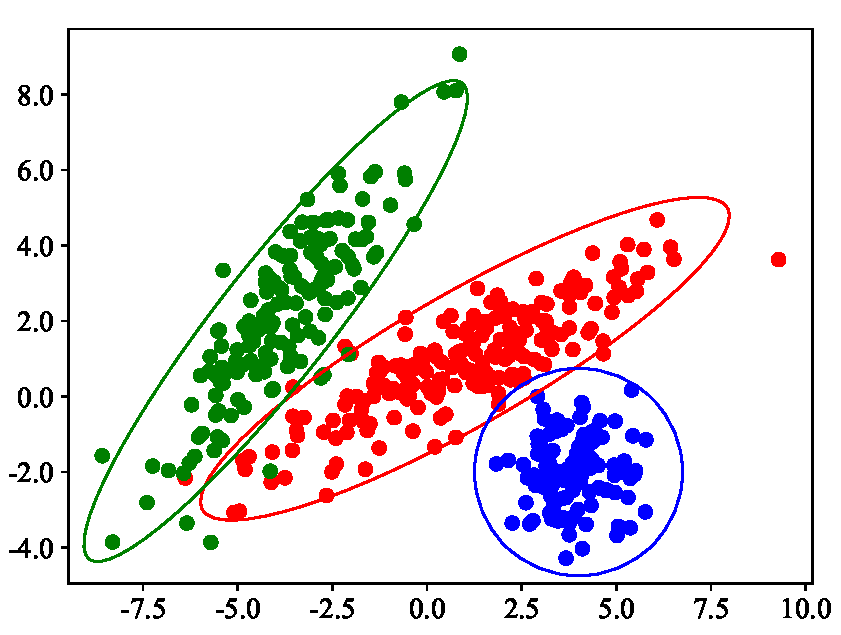
\includegraphics[width=0.7\textwidth]{obrazky/gmm.pdf}
	\caption{Rozdělení dat do~3~shluků algoritmem GMM}
	\label{gmm-img}
\end{figure}

\subsection{SOM}
Algoritmus SOM (Self-Organizing-Maps), nebo také Kohonenova mapa podle jeho tvůrce, je speciální typ neuronové sítě. Produkuje nízkodimenzionální diskretizovanou reprezentaci vstupních dat v~podobě mapy~\cite{som-web}. Od~jiných neuronových sítí se liší především tím, že se neučí na~základě opravy chyb, jako je tomu například u~gradientního sestupu, nýbrž určité sousední funkce, která zachovává zvolenou topologii mapy~\cite{som-web}. Topologie mapy neuronů se určuje na začátku algoritmu a typicky se volí obdélníková nebo hexagonální \cite{data-science-concepts-and-practice}. Jednotlivé neurony zde prakticky specifikují shluky. Práce \emph{Brief Review of~Self-Organizing Maps} \cite{som-article} algoritmus popisuje následovně:

\begin{enumerate}
    \item Náhodně se inicializují váhy neuronů každému vstupnímu bodu (viz. w\textsubscript{ij} na~obr.~\ref{som-img}).
    \item Náhodně se vybere jeden ze vstupních vektorů.
    \item Zvolí se vítězný neuron nejčastěji na~základě eukleidovské vzdálenosti od~prvků vybraného vstupního vektoru.
    \item Upraví se váhy neuronů zmíněnou sousední funkcí.
    \item Opakuje se od~bodu 2, dokud neskončí trénování.
\end{enumerate}

Úprava vah a sousední funkce zde nejsou rozebírány, neboť by si vzhledem k~jejich různým typům a složitosti zasloužily samostatnou kapitolu. Podstatné však je, že kromě váhy vítězného neuronu budou vylepšeny i váhy sousedních neuronů v~závislosti na~jejich vzdálenostech od~vítěze.

\begin{figure}[hbt]
	\centering
	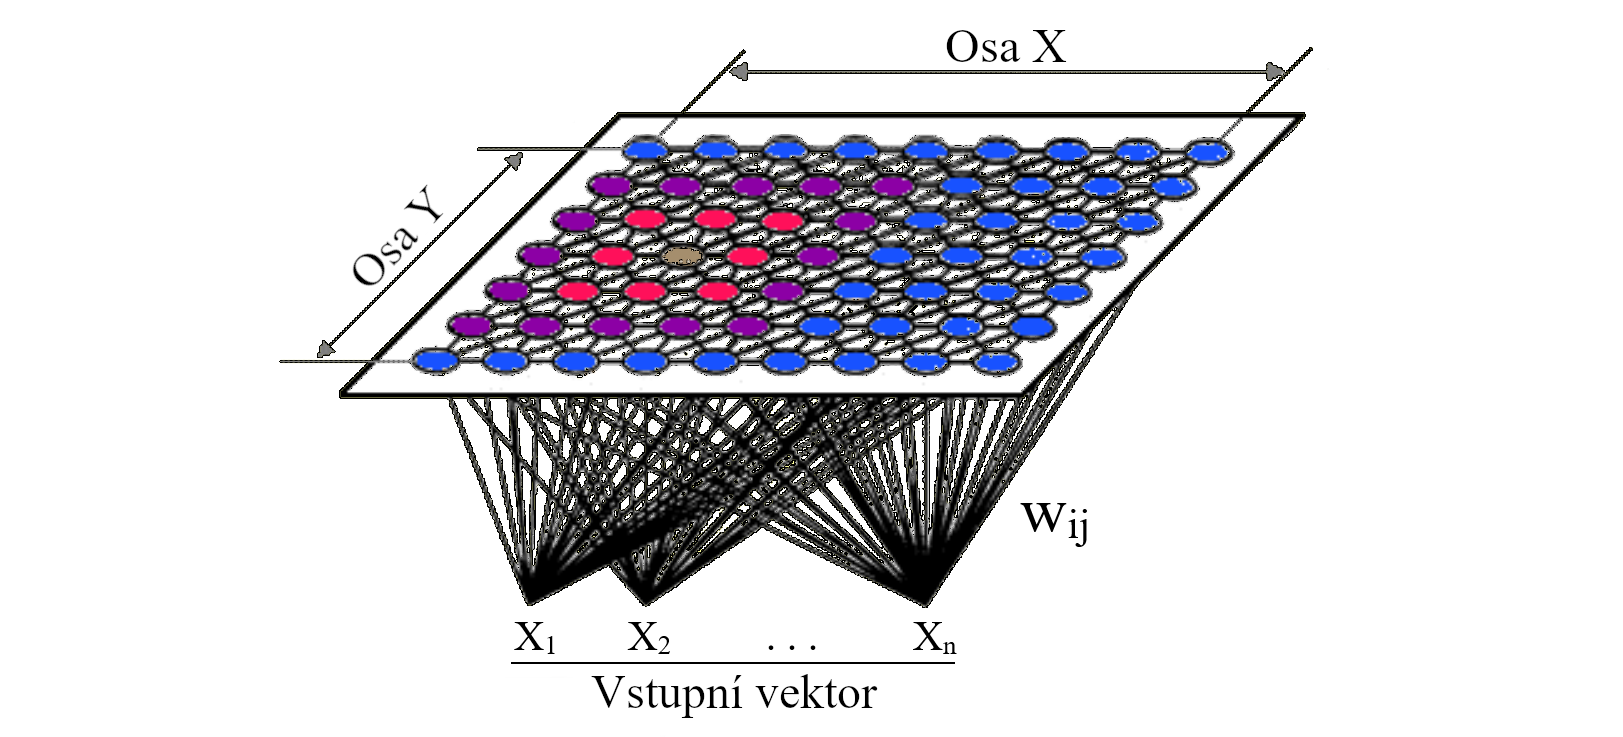
\includegraphics[width=0.85\textwidth]{obrazky/som.png}
	\caption{Ukázka propojení vstupů s~neurony a jejich váhami v~SOM (upraveno z~\cite{som-web})}
	\label{som-img}
\end{figure}

\subsection{DBSCAN}
Zkratka tohoto algoritmu znamená Density based spatial clustering of applications with noise, nebo-li prostorové shlukování aplikací s~šumem na~základě hustoty. DBSCAN je velmi rychlý algoritmus a jeho přednostmi jsou, že snadno odhalí šum a není třeba dopředu znát počet shluků. Tato informace totiž velmi často není známá. Jediné, co je třeba určit, je v~podstatě definice hustoty. Typicky se hustota měří v~kruhovém prostoru kolem bodů, a~proto je zapotřebí zvolit jisté \textepsilon, což není nic jiného, než poloměr onoho kruhu \cite{data-science-concepts-and-practice}. Druhým parametrem je minimální počet bodů, od~kterého se prostor považuje za~hustý \cite{data-science-concepts-and-practice}. Tento parametr bude dále v~práci značen jako MinPts z~anglického \uv{minimum points}. Pro každý bod se poté určí, zda leží v~husté oblasti, nebo ne. Dle literatury \cite{data-science-concepts-and-practice} se body dělí na 3 typy: 

\begin{itemize}
  \item \emph{Jádrové body} --- Mají dostatečný počet sousedů, jsou proto v~husté oblasti.
  \item \emph{Krajní body} --- Nemají dostatek sousedů, nicméně stále leží v~dosahu \textepsilon\space některého z~jádrových bodů, a~proto jsou ještě členy shluku.
  \item \emph{Šum} --- Nemá dostatek sousedů ani neleží v~dosahu \textepsilon\space některého z~jádrových bodů. Není přiřazen žádnému shluku.
\end{itemize}

Jak lze vidět na~obrázku~\ref{dbscan-vs-k-means-img}, shlukování na~základě hustoty lépe seskupí body tvořící útvary než jiné algoritmy. Nevýhodou algoritmu je však to, že nedokáže rozpoznat shluky různých hustot \cite{data-science-concepts-and-practice}. De~facto data rozděluje pouze na husté a řídké.

\begin{figure}[hbt]
	\centering
	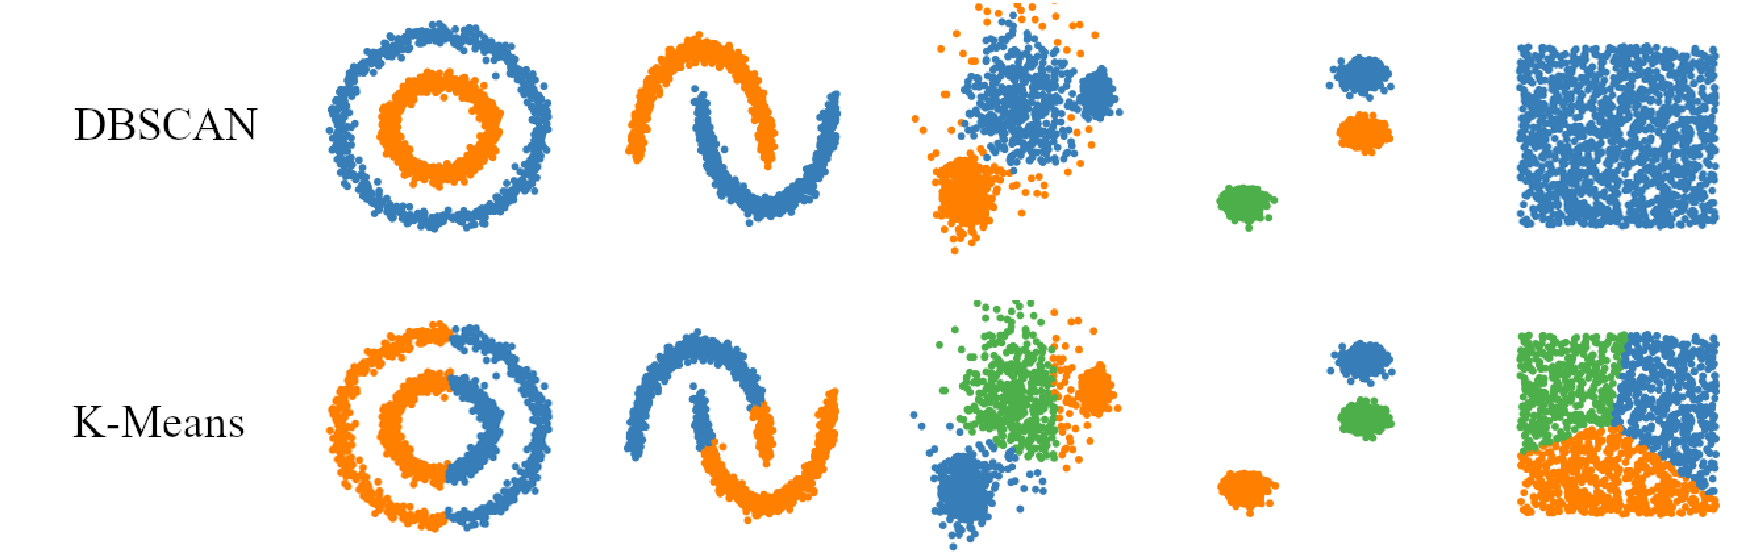
\includegraphics[width=0.83\textwidth]{obrazky/dbscan-vs-k-means.pdf}
	\caption{Porovnání shlukování algoritmy DBSCAN a K-Means (upraveno z~\cite{dbscan-vs-k-means})}
	\label{dbscan-vs-k-means-img}
\end{figure}

\subsection{HDBSCAN}
HDBSCAN (hierarchický DBSCAN) je rozšíření DBSCAN algoritmu používající hierarchické shlukování. Algoritmus je poměrně komplexní a skládá se z~mnoha kroků. Nejprve je potřeba zvolit metriku vzdálenosti mezi body. Nelze tu použít klasickou eukleidovskou vzdálenost, neboť není cílem shlukovat body, jež jsou si pouze eukleidovsky blízké, nýbrž musí být zároveň i husté~\cite{hdbscan-video}. K~tomu slouží tzv. vzdálenost vzájemné dosažitelnosti (mutual reachability distance MRD), kterou lze spočítat pomocí vzorce~\ref{mrd-rovnice}~\cite{hdbscan}:

\begin{equation}
\label{mrd-rovnice}
d_{mrd}(a,b) = max\{\epsilon_a, \epsilon_b, d(a,b)\}
\end{equation}

Hodnoty \emph{a,b} jsou dané body, \textepsilon\space je poloměr oblasti jako u~DBSCANu. Není však nastaven ad~hoc, nýbrž se jedná o~vzdálenost ke~\emph{k}-tému sousedu. Funkce \emph{d()} je klasická eukleidovská vzdálenost dvou bodů.

Pro vytvoření hierarchického dendrogramu nechť je dán graf, jehož vrcholy jsou jednotlivé body a hrany mají váhy rovny vzdálenostem mezi nimi. Zvolí se práh s vysokou hodnotou, jež se bude v~dalších průchodech postupně snižovat~\cite{hdbscan}. Během průchodů se odstraňují hrany s~váhou vyšší než je aktuální prahová hodnota, čímž se graf začne rozpojovat do~propojených komponent a tím vznikat hierarchický strom~\cite{hdbscan}. Vzhledem k~tomu, že existuje \emph{n\textsuperscript{2}} hran, měl by algoritmus asymptotickou složitost \emph{O(n\textsuperscript{2})}, a~proto je graf pro~zrychlení dopředu zredukován na~minimální kostru (obr.~\ref{hdbscan-dendrogram-img}a) Jarníkovým (Primovým) nebo Borůvkovým algoritmem~\cite{hdbscan}. Výsledný dendrogram (obr.~\ref{hdbscan-dendrogram-img}b) poté vznikne spojováním hran, dokud se nedojde ke kořenu.

\begin{figure}[hbt]
    \centering
    \subfloat[\centering Minimální kostra grafu]{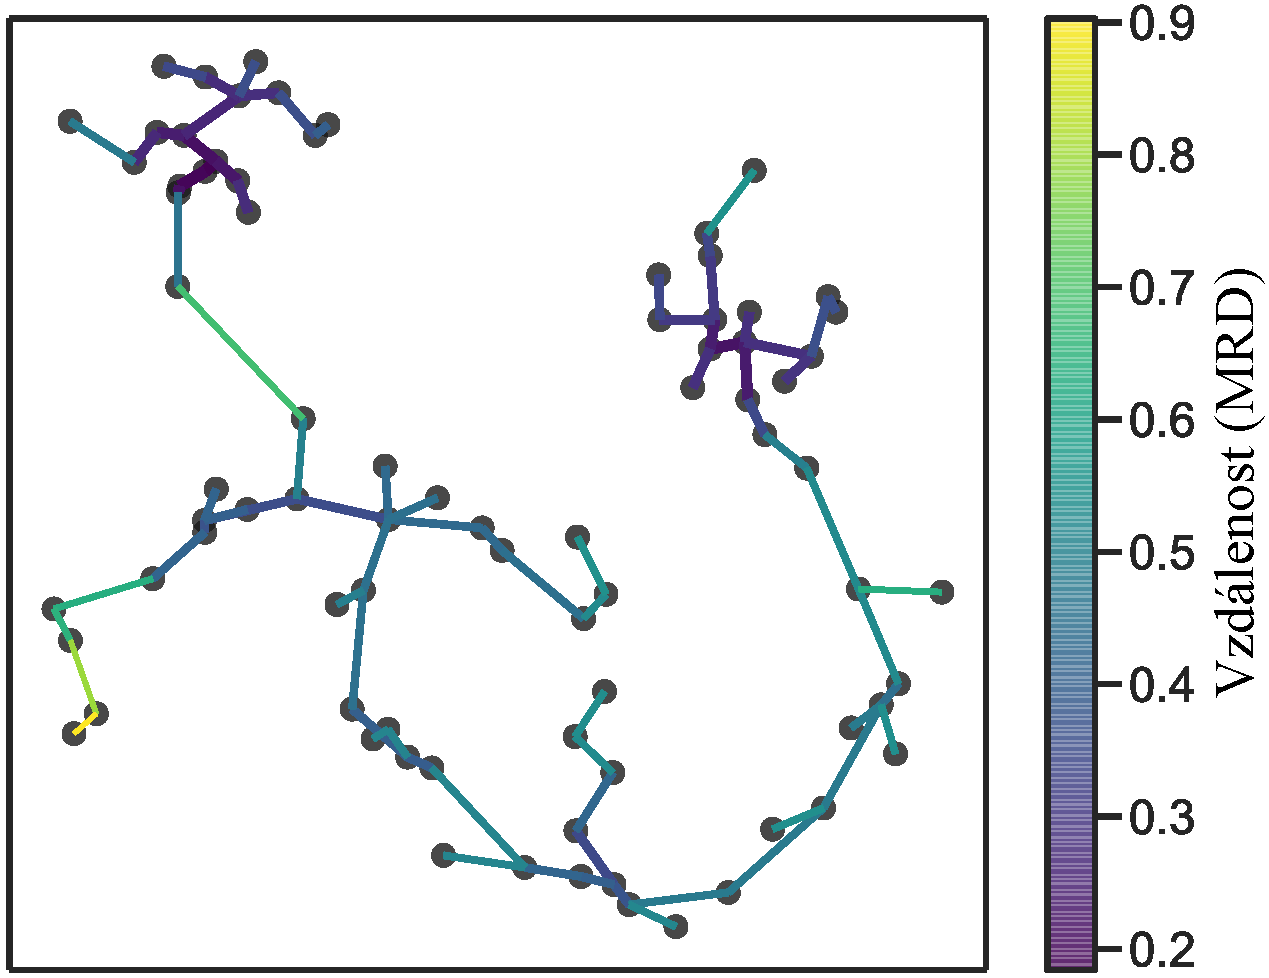
\includegraphics[width=6.9cm]{obrazky/hdbscan-tree.pdf} }
    \subfloat[\centering Výsledný dendrogram]{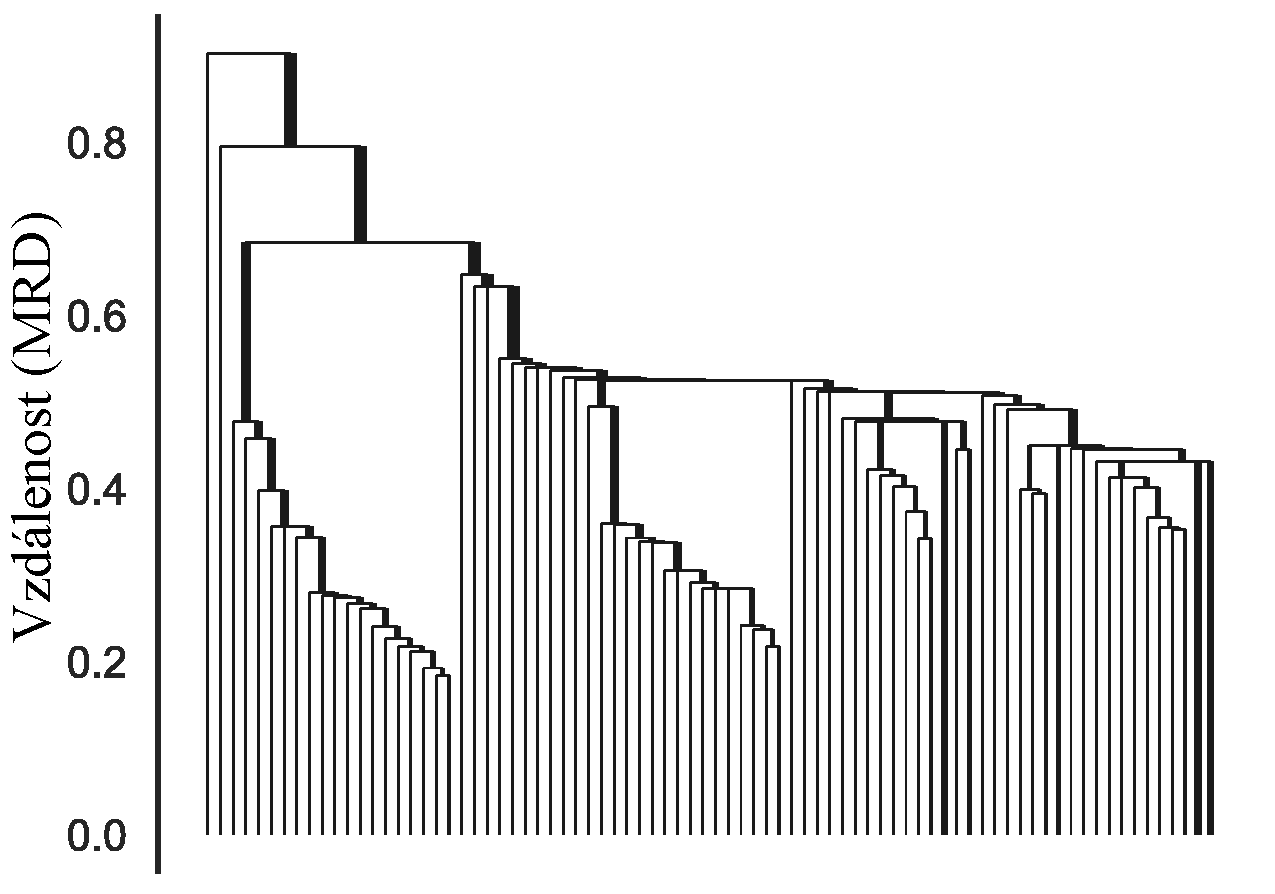
\includegraphics[width=7.7cm]{obrazky/hdbscan-dendrogram.pdf} }
    \caption{Vytvořený dendrogram s~využitím minimální kostry algoritmem HDBSCAN}
    \label{hdbscan-dendrogram-img}
\end{figure}

V~tomto bodě jsou již známy shluky, nicméně v~praxi není žádoucí reprezentace hierarchickou strukturou, nýbrž sadou daných shluků. DBSCAN by zde vytyčil práh minimálních bodů pro hustou oblast, dendrogram tímto prahem prořízl, shluky pod čarou zahodil jako šum, zbytek si ponechal a skončil~\cite{hdbscan}.
HDBSCAN však napravuje nedostatek DBSCANU ve variabilitě hustot a dendrogram prořízne v~různých místech. Jak se to provede? Dopředu se určí minimální velikost shluku a při~dělení shluku se s~touto porovná velikost obou potomků~\cite{hdbscan}. Pokud jsou oba větší, dělení je platné a ve~stromu vzniknou nové větve~\cite{hdbscan}. V~opačném případě se potomci zahodí jako šum~\cite{hdbscan}. Tím vznikne kondenzovaný strom~\ref{hdbscan-result-img}.

Nyní již zbývá pouze zvolit výsledné shluky. Prvním pravidlem je, že pokud se již některý vybere, nesmí se použít žádný z~jeho potomků~\cite{hdbscan}. Volba shluků se provádí na~základě jejich stability, jejímuž výpočtu~\ref{stabilita-rovnice} slouží zvláštní proměnná \(\lambda = 1 / d_{mrd}\), kde vzdálenost \emph{d\textsubscript{mrd}} je hodnota osy y v~dendrogramu~\ref{hdbscan-dendrogram-img}(b)~\cite{hdbscan}.

\begin{equation}
\label{stabilita-rovnice}
S = \sum_{i\in shluk}(\lambda_i - \lambda_{v})
\end{equation}

\textlambda\textsubscript{i} je zde lambda jednotlivých bodů shluku a \textlambda\textsubscript{v} pak lambda vzniku shluku. Následně se jako vybrané shluky zvolí listy stromu a postupuje se ke~kořenu. Spočítá se stabilita vybraných shluků a jejich rodičů. Pokud je stabilita rodiče větší než suma stabilit potomků S\textsubscript{p}, rodič se stává novým zvoleným prvkem~\cite{hdbscan}. V~opačném případě se rodiči nastaví hodnota stability na~S\textsubscript{p}~\cite{hdbscan}.

\begin{figure}[hbt]
	\centering
	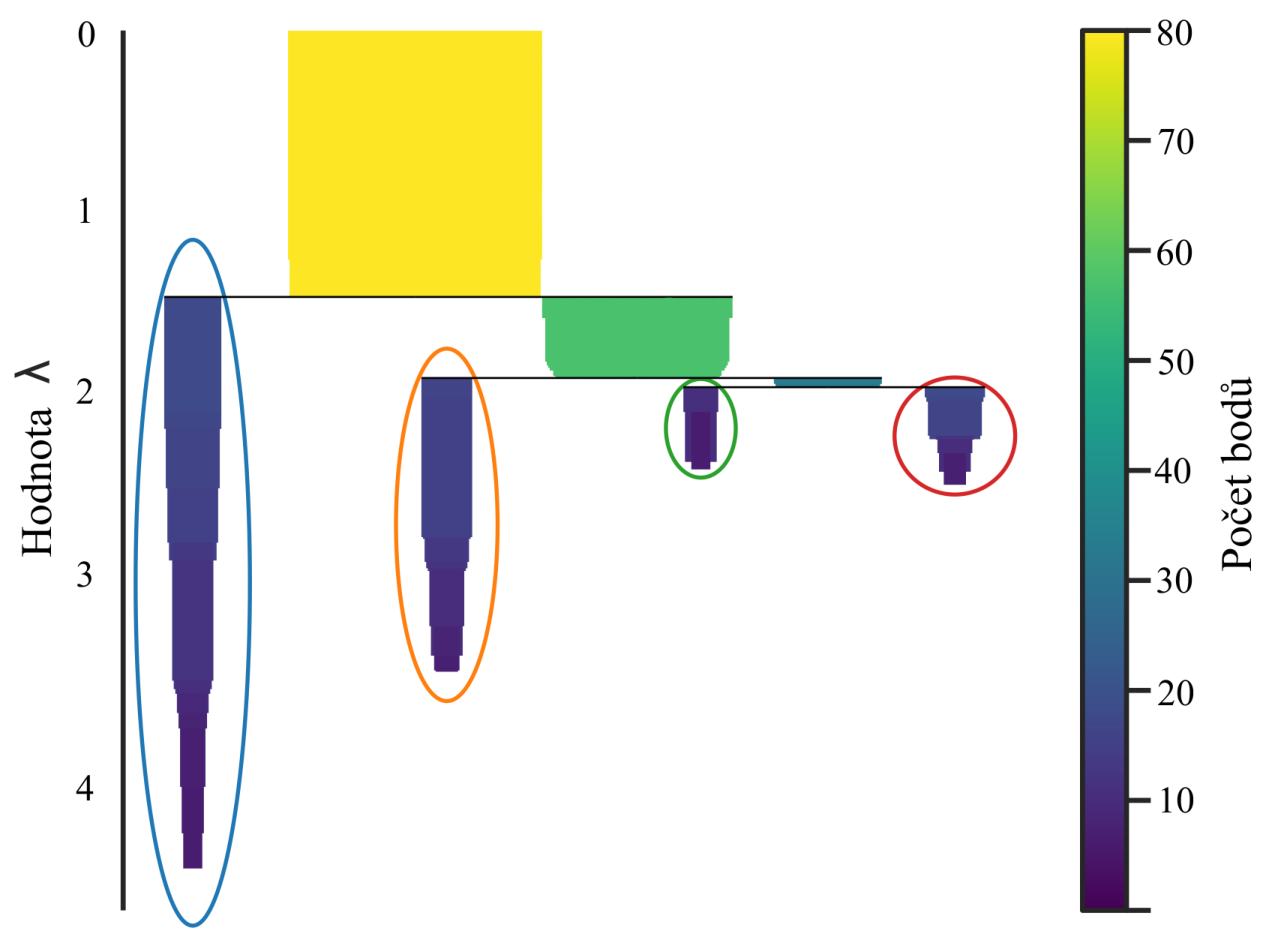
\includegraphics[width=0.7\textwidth]{obrazky/hdbscan-condensed-tree.pdf}
	\caption{Kondenzovaný strom s vyznačenými výslednými shluky}
	\label{hdbscan-result-img}
\end{figure}

Výsledkem HDBSCANu jsou shluky podobné těm od~DBSCANu na obrázku~\ref{dbscan-vs-k-means-img} s~tím rozdílem, že dokáže pojmout více stupňů hustot. Navíc vzhledem ke~znalosti hodnoty \textlambda\textsubscript{i} je schopen vytvořit měkké skóre určující, jak moc bod k~danému shluku patří~\cite{hdbscan}. Při~zanedbání určitých konstant lze jeho časovou složitost vnímat jako \emph{O(NlogN)}~\cite{hdbscan-video}, což ho řadí mezi nejrychlejší shlukovací algoritmy k~dispozici.

\subsection{OPTICS}
K~algoritmům založených na~hustotě patří také OPTICS (Ordering Points to Identify Cluster Structure). Jedná se o~příbuzný algoritmus DBSCANu, jenž řeší problém variability hustoty a zjednodušuje nalezení počátečních parametrů definující jádrové body. Kromě jádrové vzdálenosti \textepsilon\space pracuje ještě s~tzv. dosažitelnou vzdáleností (reachability distance RD)~\cite{optics}, která je zjednodušením MRD u~HDBSCANu. Jedná se o~vzdálenost mezi jádrovým bodem \emph{p} a nějakým jiným bodem \emph{q}~\cite{optics}. Platí pro~ni vztah~\ref{rd-rovnice}~\cite{optics}:

\begin{equation}
\label{rd-rovnice}
d_{rd}(p,q) = max\{\epsilon_p, d(p,q)\}
\end{equation}

V~rovnici je opět \textepsilon\textsubscript{p}\space poloměrem oblasti \emph{p} jako u~DBSCANu a funkce d() eukleidovskou vzdáleností.

Algoritmus spočívá v~tom, že se vypočítají dosažitelné vzdálenosti a data se poté seřadí tak, aby spolu blízké body sousedily~\cite{optics}. Při~vykreslení RD (obr.~\ref{optics-img}) lze shluky snadno identifikovat jako taková U~\cite{optics}, neboť na~okrajích shluku jsou RD logicky větší.

\begin{figure}[hbt]
	\centering
	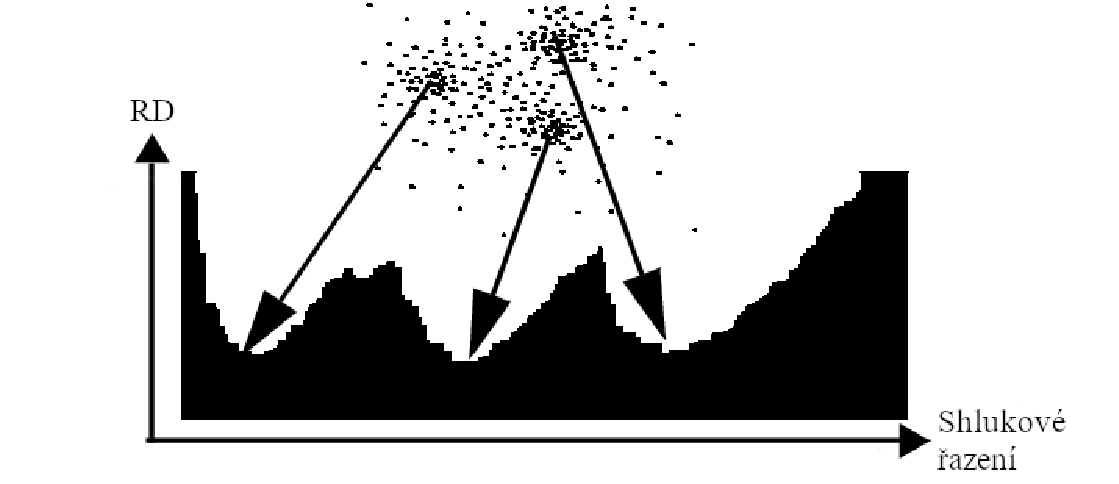
\includegraphics[width=0.9\textwidth]{obrazky/optics.pdf}
	\caption{Identifikace shluků z RD grafu (upraveno z~\cite{optics})}
	\label{optics-img}
\end{figure}

\section{Statistické metody}
Často k~detekci anomálií není třeba žádných zvláštních algoritmů a bohatě stačí statistické výpočty. Z~nich ostatně mnoho algoritmů vychází. Hlavní výhodou tohoto přístupu je jeho rychlost a jednoduchost. Na~druhou stranu má ale jen omezený rozsah použitelnosti.

\subsection{Pravděpodobnostní rozložení}
Předpokládají-li se data z~určitého rozložení pravděpodobnosti bez ohledu na~typ, lze velmi snadno detekovat outliery v~daném datasetu. Jednoduše stačí konkrétní datový bod dosadit do~příslušného vzorce, aby se zjistilo, zda do daného rozložení patří. Snadno lze výpočet modifikovat i pro~přidání případné tolerance.

Nechť se uvažuje například normální rozložení. To je definováno střední hodnotou \(\mu\) a směrodatnou odchylkou \(\sigma\). Pro toto rozložení platí pravidlo 3-sigma (obr.~\ref{3-sigma-img}), které říká, že cca 99.7~\% bodů Gaussova rozložení se nachází ve~vzdálenosti \(3\sigma\) od~jeho středu~\cite{3-sigma}. Z~toho vyplývá, že prakticky všechny vzdálenější body lze považovat za~outliery. Pravidlo \mbox{3-sigma} má navíc tu vlastnost, že vzdálenost \(2\sigma\) přibližně udává 95. percentil. Ten má mnoho využití v~různých sférách. Pro~některé aplikace umělé inteligence jím lze například čistit dataset od~outlierů. V~těch zbylých 5~\% se sice ještě nachází platná data, proto to nemusí být použitelné přímo pro~detekci, nicméně většinu outlierů to oddělá a chybějící krajní data, byť platná, kvalitu datasetu již tolik nemusí ovlivnit.

\begin{figure}[hbt]
	\centering
	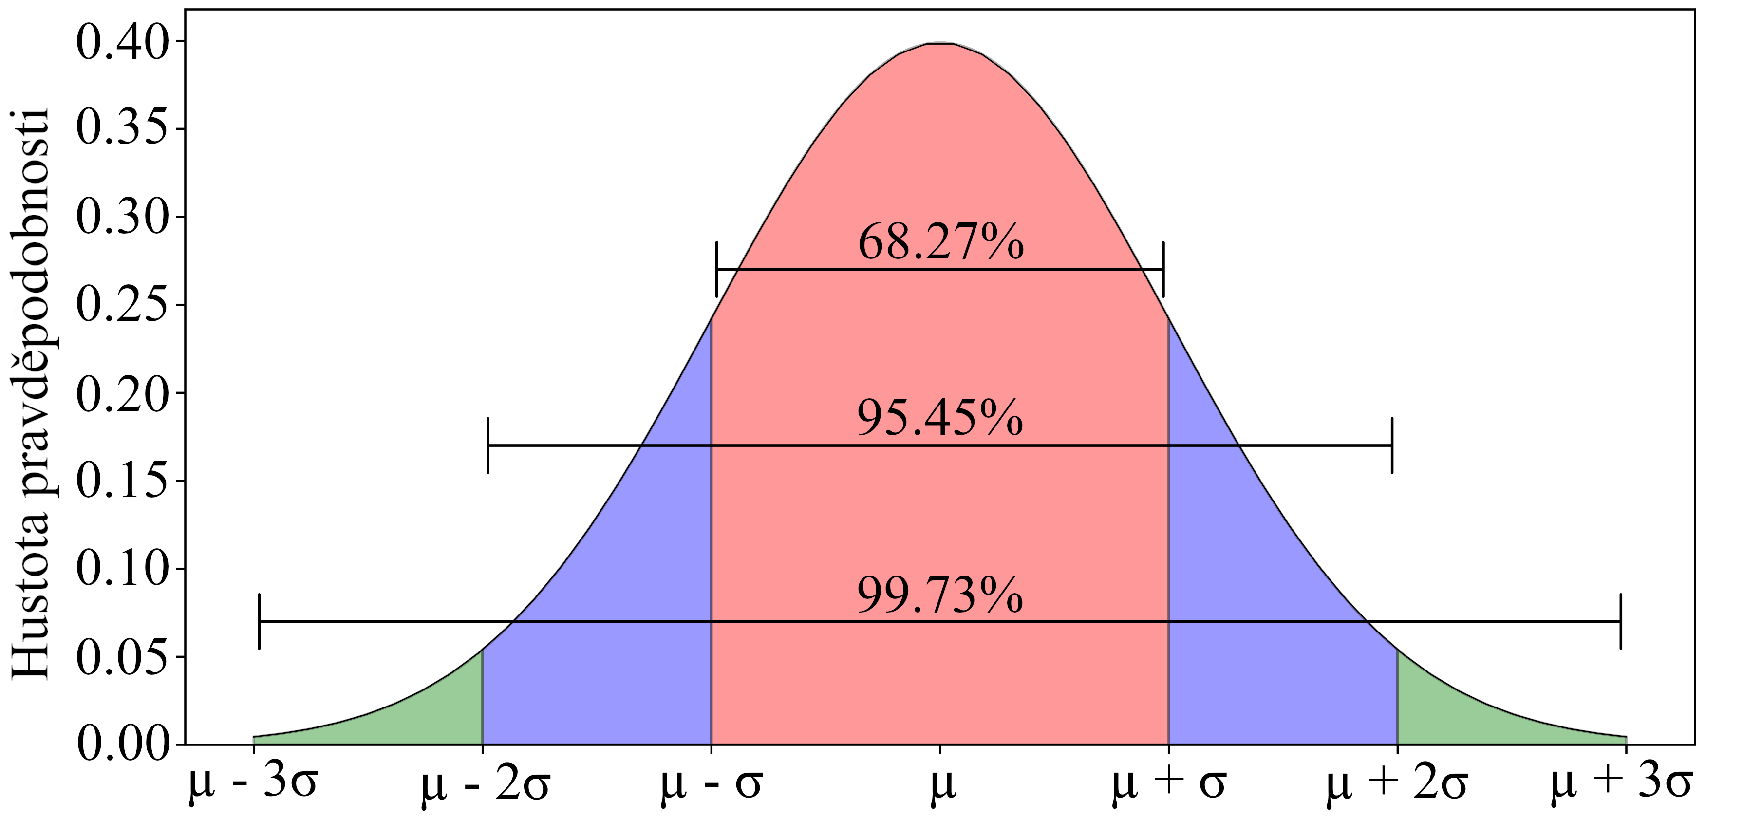
\includegraphics[width=0.85\textwidth]{obrazky/3-sigma.pdf}
	\caption{Pravidlo 3-Sigma Gaussova rozložení (upraveno z~\cite{3-sigma})}
	\label{3-sigma-img}
\end{figure}

\subsection{MAD}
Median Absolute Deviation (MAD), nebo-li medián absolutní odchylky, je velmi robustní statistické metoda využívaná k~měření variability dat~\cite{mad}. Lze ji vyjádřit jednoduchým vzorcem~\ref{mad-rovnice}:

\begin{equation}
\label{mad-rovnice}
MAD(X) = median({|x_i - median(X)|})
\end{equation}

V~podstatě se jen vypočítá medián datasetu X, pro~každou hodnotu x\textsubscript{i} z~datasetu X se spočítá odchylka od~onoho mediánu a jako výsledek se vezme medián absolutních hodnot těchto odchylek~\cite{mad}. V~detekci anomálií se často využívá pro~porovnávání časových řad~\cite{mad}. Jestliže se MAD bodu některé řady liší v~porovnání s~body v~ostatních řadách ve~stejném časovém úseku o~více než předem stanovenou mez, lze bod považovat za~outlier. Pokud řadu tvoří více než určité procento outlierů, celá řada je pak outlier.

\subsection{Z-skóre a modifikované z-skóre}
Z-skóre lze vnímat jako standardizované normální rozložení určitého datasetu se vzorcem~\ref{zscore-rovnice}. Vyjadřuje odchýlení jednotlivých bodů od~průměru v~jednotkách směrodatné odchylky.

\begin{equation}
\label{zscore-rovnice}
Z = \dfrac{X - \mu}{\sigma}
\end{equation}

Jeho nepřesnost však spočívá v~tom, že outliery silně ovlivňují nejen průměrnou hodnotu, nýbrž i směrodatnou odchylku. Tento problém řeší tzv.~modifikované z-skóre, které používá robustnější parametry, konkrétně tedy medián místo průměru a MAD místo směrodatné odchylky~\cite{z-score}. Výsledek pak ještě dle vzorce~\ref{modifikovane-zscore-rovnice} násobí normalizační konstantou 0.6745~\cite{z-score}.

\begin{equation}
\label{modifikovane-zscore-rovnice}
Z = 0.6745\times\dfrac{X - median(X)}{MAD(X)}
\end{equation}

Dále je pouze třeba vymezit hraniční skóre, nad~kterým budou prvky považovány za~outliery. Cena za~rychlost, robustnost a jednoduchost této metody je však předpoklad alespoň přibližného normálního rozložení zpracovávaných dat.

\section{Rozhodovací stromy}
Typickým použitím rozhodovacích stromů je klasifikační nebo regresní analýza objektů na~základě jejich vlastností. Strom se vytváří dělením zdrojové množiny dle hodnot parametrů jejích objektů na~podmnožiny, jež se stávají zdrojovými množinami pro~další větvení~\cite{decision-trees}. Výběr vhodných parametrů pro~co nejúčinější dělení se provádí specifickou funkcí pro~daný problém. Častým způsobem je například výpočet tzv.~informačního zisku na~základě entropie~\cite{decision-trees}. Rozhodovací stromy jsou jednou z~nejstarších a nejběžnějších metod pro~získání informací z~dat nejen v~oblasti strojového učení. Jak je však lze využít k~detekci anomálií?

\subsection{Isolation forest}
\label{isolation-forest}
Tvůrci algoritmu Isolation forest (česky izolační les) ve své studii \cite{isolation-forest} tvrdí, že většina algoritmů pro~detekci anomálií pracuje na~tom způsobu, že si definují, co~je normální, a za~anomálie prohlašují ta data, jež nesplňují daná kritéria. Tyto algoritmy jsou pak podle nich optimalizované právě pro~úkol najití běžného chování, nikoliv však pro~samotnou detekci anomálií. Další nevýhodu vidí v~omezení na~nízkodimenzionální data z~důvodu výpočetní složitosti.
K~problému proto přistupují obráceně a algoritmus navrhují tak, aby se již přímo zaměřoval na~vyčlenění anomálních dat. Toho lze dosáhnout zaměřením se na~jejich obecné vlastnosti, tedy že jich je málo a jsou nějakým způsobem odlišné.

Princip fungování algoritmu není příliš složitý. Jeho cílem je odizolovat jednotlivé prvky z~datové množiny. Nechť se vezme v~úvahu dataset vykreslený na obrázku~\ref{isolation-forest-splitting-img}. Pro~každý bod se náhodně zvolí dimenze a místo, ve~kterém se provede řez, čímž se rozštěpí strom na~dvě větve~\cite{isolation-forest}. Štěpení se dále provádí, dokud se prvek neodizoluje, nebo dokud není dosaženo předem stanovené maximální výšky stromu~\cite{isolation-forest}. Anomální prvky k~odizolování potřebují méně řezů než platné.

\begin{figure}[hbt]
	\centering
	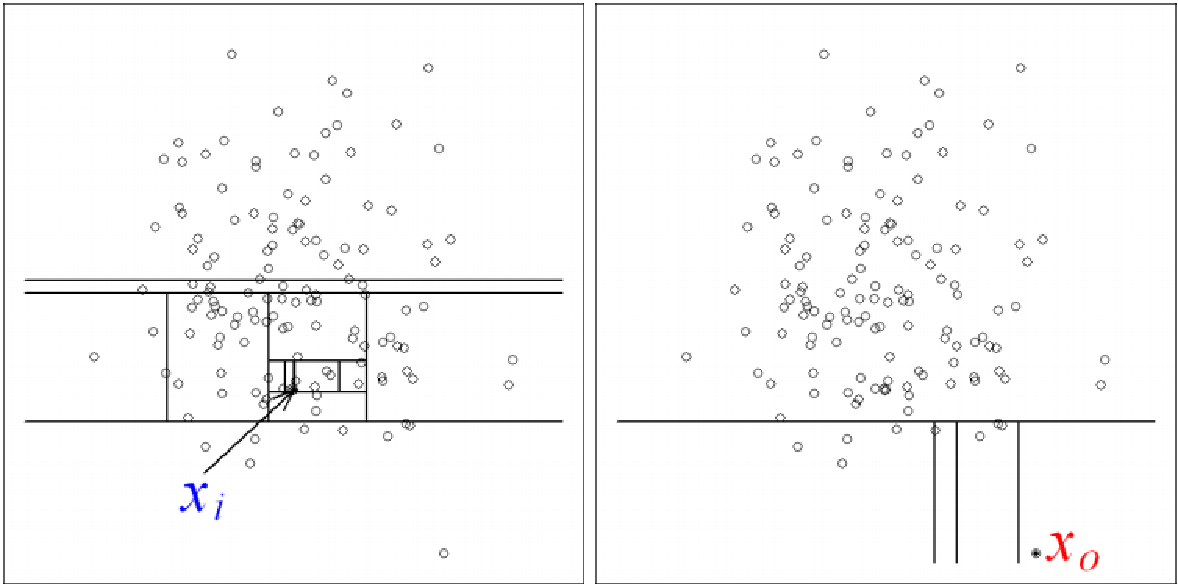
\includegraphics[width=1\textwidth]{obrazky/isolation-forest-splitting.pdf}
	\caption{Izolování prvků náhodnými řezy v~algoritmu Isolation forest (převzato z~\cite{isolation-forest})}
	\label{isolation-forest-splitting-img}
\end{figure}

Anomálie se však mohou vyskytovat ve~shlucích nebo blízko platných dat. V~takovém případě by výše zmíněný postup nebyl moc efektivní. Zde proto přichází do~hry tvorba lesa. Dataset se podvzorkuje, čímž se zmenší význam shluků a zvýrazní izolace (obr.~\ref{isolation-forest-subsampling-img})~\cite{isolation-forest}. Algoritmus se pak provádí nad~těmito redukovanými datasety. Ve~výsledku tak vzniká několik stromů (les), který každý dává vlastní výsledek. To má ty pozitivní vlastnosti, že se výrazně potlačuje přetrénování, jež zcela jistě u~některých stromů nastane, ale ne u~všech a u~každého třeba v~jiném směru. Dále je model přesnější, neboť vícero stromů se musí shodnout na~výsledku~\cite{isolation-forest}.

\begin{figure}[hbt]
    \centering
    \subfloat[\centering Původní data]{{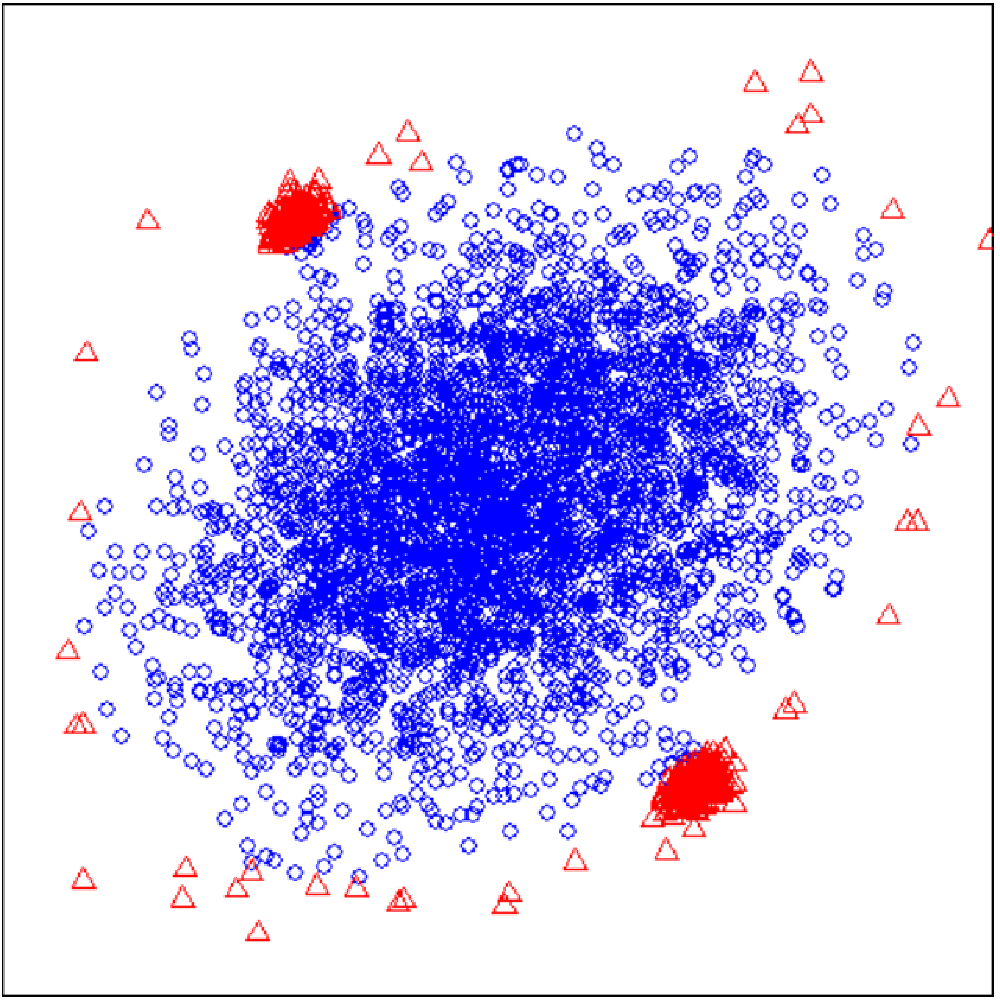
\includegraphics[width=7cm]{obrazky/isolation-forest-subsampling-1.pdf} }}
    \qquad
    \subfloat[\centering Podvzorkovaná data]{{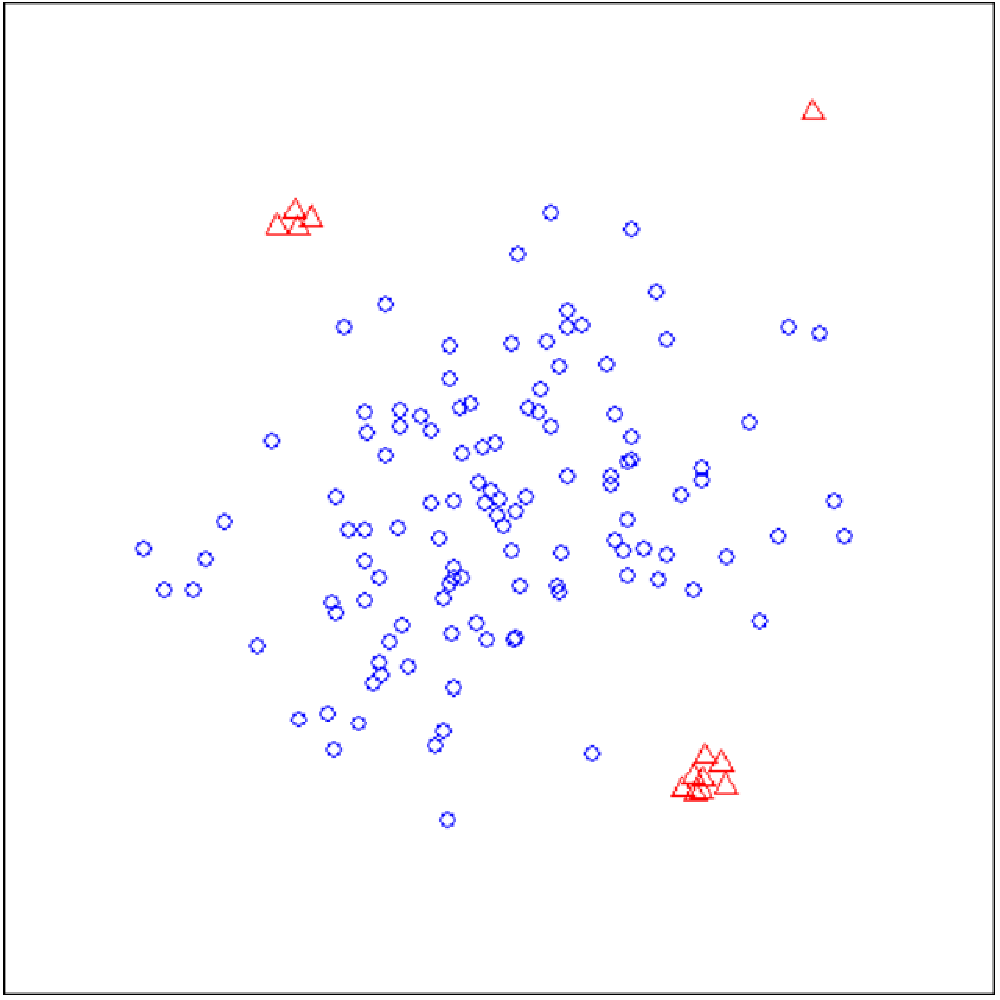
\includegraphics[width=7cm]{obrazky/isolation-forest-subsampling-2.pdf} }}
    \caption{Podvzorkovaná data snáze vytyčí anomální body (převzato z~\cite{isolation-forest}).}
    \label{isolation-forest-subsampling-img}
\end{figure}

Samotné rozhodnutí o~anomálii se provádí měkce pomocí skóre každého prvku. To závisí na~počtu řezů, tedy délce cesty k prvku ve~stromu. Hodnota skóre se pohybuje v~intervalu \(<0,1>\), lze proto snadno uvádět procentuální míru anomálnosti prvku. Dle aplikace se jen určí vhodná hranice. Práce \emph{Isolation Forest}~\cite{isolation-forest} vysvětluje skóre následovně. Prvek se skóre blízkým 1 je zcela jistě outlier. Výrazně nižší skóre než~0.5 pak indikuje naprosto běžný prvek. Jestliže však mají všechny prvky skóre blízké 0.5, pak celý dataset nevykazuje žádné výrazné anomálie.

Předními vlastnostmi algoritmu Isolation forest jsou podle literatury~\cite{isolation-forest} jeho lineární časová složitost a velmi nízké paměťové nároky. Dále se uvádí jeho vysoká rychlost v~porovnání s~jinými algoritmy, neboť nepočítá žádné vzdálenosti. Díky podvzorkování pak dokáže zpracovat velmi velká nebo i vysokodimenzionální data. V~neposlední řadě je mnohem snazší volba parametrů algoritmu než je tomu u~jiných metod. Stačí specifikovat pouze počet stromů a jejich velikost, přičemž oba tyto parametry již mají empiricky ověřené vhodné hodnoty.
